\documentclass[11pt]{report}
\usepackage[pdftex]{graphicx}
\usepackage{henrian-more}
\usepackage{amsmath}
\usepackage{subfig}
\usepackage{booktabs}
\usepackage{rotating}
\usepackage{float}

\makeHeaders{Machine Learning: Homework 3}

\begin{document}

\begin{itemize}
  \item \textbf{Email}: chrisbrown@utexas.edu
  \item \textbf{EID}: chb595
\end{itemize}

\section{Inverse Transpose}

I will show that
\[ \frac{ \partial ln|A| }{ \partial A } = (A^{-1})^T \]
% Note that $(A^{-1})^T = (A^T)^{-1}
% Multiply the term on the left side of the equation by 1:
Let the function $g(x) = |x|$, and the function $g(x) = ln(x)$, and compose the two into $F(x) = f(g(x))$. The chain rule says that
\[\frac{F'(x)}{x'} = \frac{f'(g(x))}{g'} \frac{g'(x)}{x'}\]
Thus the term on the left side of the equation, \(\frac{\partial(f(g(A)))}{\partial A}\) derives to:
\[ \frac{\partial f(g(A))}{\partial g(A)} \frac{\partial g(A)}{\partial A} \]
And back in the original terms:
\[ \frac{\partial ln|A|}{\partial |A|} \frac{\partial |A|}{\partial A} \]
Now since $\frac{ln\;x}{dx} = \frac{1}{x}$, and since $\partial [constant] = 1$, and $|A|$ is just a constant, we just get:
\[ \frac{1}{|A|} \frac{\partial |A|}{\partial A} \]
The fraction on the right hand side, $\frac{\partial |A|}{\partial A}$ can alternatively be notated:
$\nabla_A |A|$, or written out as:
\[
\begin{bmatrix}
  \frac{\partial |A|}{\partial A_{11}} & \frac{\partial |A|}{\partial A_{12}} & \cdots \\
  \frac{\partial |A|}{\partial A_{21}} & \ddots & \cdots \\
  \vdots & \vdots & \frac{\partial |A|}{\partial A_{mn}} \\
\end{bmatrix}
\]
As in Andrew Ng's course notes, we define the adjoint as
\[(\text{adjoint}(A))_{ij} = (-1)^{i+j}|A_{\backslash j,\backslash i}|\]
And keep that definition of the determinant:
\[|A| = \sum^n_{i=1} a_{ij} (-1)^{i+j}|A_{\backslash i,\backslash j}|\]
Let's transpose the matrix in the definition of the adjoint:
\begin{align*}
  (\text{adjoint}(A))_{ij} = (-1)^{i+j}|(A^T)_{\backslash i,\backslash j}|
  & & \text{or} & &
  (\text{adjoint}(A^T))_{ij} = (-1)^{i+j}|(A)_{\backslash i,\backslash j}|
\end{align*}
And so we can redefine the determinant as:
\[|A| = \sum^n_{i=1} a_{ij}\, \text{adjoint}(A^T)\]
And now it's relatively clear why $\nabla_A |A| = \text{adjoint}(A)$, so we have
\begin{align*}
  \frac{1}{|A|} \frac{\partial |A|}{\partial A}
  \quad=\quad
  \frac{1}{|A|} \nabla_A |A|
  \quad=\quad
  \frac{1}{|A|} \text{adjoint}(A) 
  \quad \overset{?}{=}\; (A^{-1})^T
\end{align*}
% xxx clarify...
% (My intuition about it is that --- errmm, I don't really have any intuition about this one.



% By definition, $|I| = 1$, and so $|AA^{-1}| = 1$, and we've also assumed that $|A||B| = |AB|$, so we see that $|A||A^{-1}| = 1$.
\medskip \noindent
By definition of the determinant, \[\text{adjoint}(A)A = |A|I\] % A\text{adjoint}(A) =
This can be reordered:
\begin{align*}
  \text{adjoint}(A)A = |A|I
  & & \rightarrow & &
  \frac{1}{|A|}\text{adjoint}(A)A = I
\end{align*}
Since $|A|$ is a scalar, it doesn't really matter where it goes. Then
\begin{align*}
  \frac{1}{|A|}\text{adjoint}(A)AA^{-1} = IA^{-1}
  & & \rightarrow & &
  \frac{1}{|A|}\text{adjoint}(A) = A^{-1}
\end{align*}
Almost done, but it seems like we're missing a transpose. However, note that we can write out our current progress with all of our values as determinants (since $\nabla_A |A| = \text{adjoint}(A)$):
\[\frac{1}{|A|}\nabla_A |A| = A^{-1}\]
But we know that
\begin{align*}
  |A| = |A^T|
  & & \text{and} & &
  (A^{-1})^T = (A^T)^{-1}
\end{align*}
So we can write out, finally:
\begin{align*}
  \frac{1}{|A|}\nabla_A |A| = (A^{-1})^T
  & & \text{and} & &
  \left(
    \frac{ \partial ln|A| }{ \partial A } =
  \right)
  \frac{1}{|A|}\frac{\partial |A|}{\partial A} = (A^{-1})^T
\end{align*}

\section{Positive eigenvalues}

% For a matrix $A$, eigenvalues $\Lambda$, and eigenvectors $X$, by definition:
% \[ AX = X\Lambda \]
For a matrix $A$ and any eigenvector $x$ and eigenvalue $\lambda$:
\[ Ax = \lambda x \]
A (square) positive definite matrix $A$ is defined as: $x^TAx > 0$, where $x$ is any vector of the same width as $A$ (and $x$ is non-zero).
We wish to show that if $x$ is an eigenvector of $A$, which is positive definite, then the corresponding eigenvalue $\lambda$ is positive.

First, multiply both sides of the eigenvector equation by $x^T$:
\[ x^TAx = x^T\lambda x \]
Because we presume that $A$ is positive definite, and we are dealing with non-zero eigenvectors ($x$), we see that the left side of this equation must be greater than zero, and so must be the right side:
\[ x^T\lambda x > 0 \]
Now, since $\lambda$ is just a scalar number, we can move it over:
\[ x^Tx\lambda > 0 \]
A vector multiplied by its transpose is a sum of squares:
\[
  \begin{bmatrix}
    x_1 & x_2 & x_3 & x_4
  \end{bmatrix}
  \begin{bmatrix}
    x_1 \\ x_2 \\ x_3 \\ x_4
  \end{bmatrix}
  =
  x_1^2 + x_2^2 + x_3^2 + x_4^2
\]
We're only dealing with real numbers, so our squares must be non-negative. But we've also asserted that our vector $x$ is non-zero, so the sum of our squares must be positive (non-zero). We declare that $c = x^Tx$,
\[ c\lambda > 0 \]
And since we've shown that $c > 0$, we can safely divide both sides by $c$ without flipping the equality, and we're done:
\[ \lambda > 0 \]
Of course, this works for any eigenvalue $\lambda$, since it works for the general case.


\section{Matrix Algebra}

We will show:
\[ (A + BD^{-1}C)^{-1} = A^{-1} - A^{-1}B(D + CA^{-1}B)^{-1}CA^{-1} \]
Begin by multiplying both sides by $(A + BD^{-1}C)$
\[ (A + BD^{-1}C)^{-1}(A + BD^{-1}C) \overset{?}{=} (A^{-1} - A^{-1}B(D + CA^{-1}B)^{-1}CA^{-1})(A + BD^{-1}C) \]
The left side reduces to unity:
\[ I \overset{?}{=} (A^{-1} - A^{-1}B(D + CA^{-1}B)^{-1}CA^{-1})(A + BD^{-1}C) \]
Factor out the $A^{-1}$ on the right side:
\[ I \overset{?}{=} (A^{-1})
  (1 - B(D + CA^{-1}B)^{-1}CA^{-1})
  (A + BD^{-1}C)
\]
Now distribute the $(A + BD^{-1}C)$ term.
\[ I \overset{?}{=} (A^{-1})(
  A + BD^{-1}C
  - B(D + CA^{-1}B)^{-1}CA^{-1}A
  - B(D + CA^{-1}B)^{-1}CA^{-1}BD^{-1}C
)\]
Simplify out $A^{-1}A$.
\[ I \overset{?}{=} (A^{-1})(
  A + BD^{-1}C
  - B(D + CA^{-1}B)^{-1}C
  - B(D + CA^{-1}B)^{-1}CA^{-1}BD^{-1}C
)\]
Factor out $B$ to the left, and $C$ to the right.
\[ I \overset{?}{=} (A^{-1})(
  A + B(
      D^{-1}
      - (D + CA^{-1}B)^{-1}
      - (D + CA^{-1}B)^{-1}CA^{-1}BD^{-1}
      )C
)\]
Factor out $(D + CA^{-1}B)^{-1}$:
\[ I \overset{?}{=} (A^{-1})(
  A + B(
      D^{-1}
      - (D + CA^{-1}B)^{-1}
        (I + CA^{-1}BD^{-1})
      )C
)\]
And inject a $DD^{-1}$:
\[ I \overset{?}{=} (A^{-1})(
  A + B(
      D^{-1}
      - (D + CA^{-1}B)^{-1}
        (I + CA^{-1}BD^{-1})DD^{-1}
      )C
)\]
And distribute towards the left:
\[ I \overset{?}{=} (A^{-1})(
  A + B(
      D^{-1}
      - (D + CA^{-1}B)^{-1}
        (D + CA^{-1}BD^{-1}D)D^{-1}
      )C
)\]
The $D^{-1}D$ cancels to $I$:
\[ I \overset{?}{=} (A^{-1})(
  A + B(
      D^{-1}
      - (D + CA^{-1}B)^{-1}
        (D + CA^{-1}B)D^{-1}
      )C
)\]
And $(D + CA^{-1}B)^{-1}(D + CA^{-1}B)$ also cancels to $I$:
\[ I \overset{?}{=}
  (A^{-1})(A + B(D^{-1} - D^{-1})C)
\]
I'll multiply it out, just to be clear. First, $A^{-1}$:
\[ I \overset{?}{=}
  A^{-1}A + A^{-1}B(D^{-1} - D^{-1})C
\]
Simplify the left term, distribute the right:
\[ I \overset{?}{=}
  I + A^{-1}BD^{-1}C - A^{-1}BD^{-1}C
\]
Subtract $I$ from both sides:
\[ 0 \overset{?}{=}
  A^{-1}BD^{-1}C - A^{-1}BD^{-1}C
\]
Add $A^{-1}BD^{-1}C$ to both sides, and the equality is obvious.
\[ A^{-1}BD^{-1}C = A^{-1}BD^{-1}C \]


% Simplify:
% \[ I \overset{?}{=} 1 + A^{-1}BD^{-1}C - A^{-1}B(D + CA^{-1}B)^{-1}C - A^{-1}B(D + CA^{-1}B)^{-1}CA^{-1}BD^{-1}C \]


% \[ \frac{\partial ln|A|}{\partial A} \dot \frac{\partial |A|}{\partial |A|} \]

% Because $\partial |A|$ is just a scalar number, we can move it over the matrix $\partial A$:

% \[ \frac{\partial ln|A| \partial |A|}{\partial |A| \partial A} \]

\section{Lagrange Can}

For a can of radius $r$ and height $h$, we want to pick the $r$ and $h$ that maximize volume,
\[V = \pi r^2h\]
while constraining surface area to a given constant.

Because `can' suggests that the intended solid is not precisely a cylinder, I will proceed under the assumption that the solid in question is a hollow cylinder with one end missing. Of course, this only affects surface area, not volume. For simplicity, I'll assume the walls of the solid are infinitely thin.
\[ A = \pi r^2 + 2\pi rh \]
Each surface could be multiplied by two for the inside and outside of the same wall, but the end result would be the same (we would just have to divide $A$ by 2 before we use it), so I will stick with counting only the outside surfaces.

The constraint means that, since we know $A$, given $r$, we can determine $h$ (or given $h$, we can determine $r$). Now we have:
\begin{align*}
  \underset{r,h}{\text{max}}\; V = \pi r^2h & & \text{subject to} & & \pi r^2 + 2\pi rh = A
\end{align*}
One constraint means one Lagrange multiplier. We set up the optimization equation:
\[
  \underset{r,h,\lambda}{\text{max}}\;V = \pi r^2h + \lambda(\pi r^2 + 2\pi rh - A)
\]
Now we differentiate:
\begin{align*}
  V_h' &= \pi r^2 + 2\pi\lambda r &= 0 &= r + 2\lambda \\
  V_r' &= 2\pi rh + 2\pi\lambda r + 2\pi\lambda h &= 0 &= rh + \lambda r + \lambda h \\
  V_\lambda' &= \pi r^2 + 2\pi rh - A &= 0 &
\end{align*}
So from the first and second equations we have:
\begin{align*}
  r &= -2\lambda \\
  h &= \frac{-\lambda r}{r + \lambda}
\end{align*}
Merging the first and second equations produces:
\[
  h = -2\lambda
\]
And substituting these values of $r$ and $h$ into the final equation produces
\[
  0 = 4\pi\lambda^2 + 8\pi\lambda^2 - A = 12\pi\lambda^2 - A
\]
Which rearranges into
\begin{align*}
  12\pi\lambda^2 = A & & \text{and} & & \lambda = \sqrt{\frac{A}{12\pi}}
\end{align*}
% at this point, \lambda = \sqrt{\frac{A}{24\pi}} for the unopen can scenario
Multiplying this back into the equations for $r$ and $h$, we get
\[
  r = h = -2\sqrt{\frac{A}{12\pi}}
\]
It's absurd to have negative dimensions, but let's continue, to derive the volume:
\[
  V = - \frac{2A}{3}\sqrt{\frac{A}{12\pi}}
\]
Yep, it's still kind of strange, so apparently it \emph{is} important to subtract the Lagrangian component when maximizing, instead of adding. (And now I'm perplexed why the box example in class (Feb. 6) worked out just fine by adding, even though it was a maximization problem, too.)

In which case we have:
\[ \underset{r,\lambda}{\text{max}}\;V = \pi r^2h - \lambda(\pi r^2 + 2\pi rh - A) \]
And:
\begin{align*}
  V_h' &= \pi r^2 - 2\pi\lambda r                 &= 0 &= r - 2\lambda \\
  V_r' &= 2\pi rh - 2\pi\lambda r - 2\pi\lambda h &= 0 &= rh - \lambda r - \lambda h \\
  V_\lambda' &= - \pi r^2 - 2\pi rh + A           &= 0 &= \pi r^2 + 2\pi rh - A
\end{align*}
And:
\[ r = h = 2\lambda \]
And substituting into the third equation gives us the same $\lambda$,
\[ \lambda = \sqrt{\frac{A}{12\pi}} \]
But now of course we'll get positive $r$ and $h$ values:
\[ r = h = 2\sqrt{\frac{A}{12\pi}} \]
And a reasonable volume:
\[ V = \frac{2A}{3}\sqrt{\frac{A}{12\pi}} \]
For the \emph{un}opened can scenario, $r = 2\lambda$ and $h = 4\lambda$, and $\lambda = \sqrt{\frac{A}{24\pi}}$.
In which case
\[ V =
      \pi \left(2\sqrt{\frac{A}{24\pi}}\right)^2 \left(4\sqrt{\frac{A}{24\pi}}\right) =
      \frac{2A}{3}\sqrt{\frac{A}{24\pi}}
 \]









\section{Cost + Reward function optimization}

We begin with the dynamic equation (acceleration is a function of gas applied at some time):
\[ \ddot{x} = u(t) \]
and initial conditions (which simply state that we start at the beginning, with a speed of zero):
\[ x(0) = 0 \]
\[ \dot{x}(0) = 0 \]
and the reward - cost function:
\[ J = x(T) -  \int^T_0 u^2(t) dt \]
In that equation, $x(T)$ represents the distance traveled at time $T$---the bigger the better. And $\frac{1}{2} u^2(t)$ represents the acceleration (amount of gas) applied at point $t$, and the integration of that function from time = 0 to time = $T$ is the total amount of power (= gas) used between the starting point and the end time, but squared in order to encourage a gradual application of power.

$\dot{x}$ can be described as a vector of state variables, two scalars, which correspond to the derivatives of position and velocity:
\[
  \dot{x} =
  \begin{pmatrix}
    \dot{x}_1\\
    \dot{x}_2
  \end{pmatrix}
  =
  \begin{pmatrix}
    x_2\\
    -x_2 + u
  \end{pmatrix}
\]
We begin with the Hamiltonian defined as:
\[ H = \lambda^Tf(x, u) + \ell(x, u) \]
where $\lambda^T$ corresponds to the benefit part of our objective function: $x_1(T)$, $f(x, u)$ corresponds to our $\dot{x}$, and $\ell(x, u)$ corresponds to the cost part of the objective function, but without the integration, and with the negative embedded ($\ell$ for \emph{l}oss).
Our Lagrangian, $\lambda$, is just two-long:
\[ \lambda =
  \begin{pmatrix}
    \lambda_1\\
    \lambda_2
  \end{pmatrix}
\]
So we can rewrite the Hamiltonian equation as:
\begin{align*}
  H =
  \begin{pmatrix}
    \lambda_1 &
    \lambda_2
  \end{pmatrix}
  \begin{pmatrix}
    x_2 \\
    -x_2 + u
  \end{pmatrix}
  -
  \frac{1}{2}u^2
  & &
  =
  \lambda_1x_2 - \lambda_2x_2 + \lambda_2u - \frac{1}{2}u^2
\end{align*}
Now we take partial derivatives of this Hamiltonian, relative to our $x$.
\[
  \begin{pmatrix}
    -\dot\lambda_1 \\
    -\dot\lambda_2
  \end{pmatrix}
  =
  \begin{pmatrix}
    \frac{\partial H}{\partial x_1} \\
    \frac{\partial H}{\partial x_2}
  \end{pmatrix}
  =
  \begin{pmatrix}
    0 \\
    \lambda_1 - \lambda_2
  \end{pmatrix}
\]
$\phi[x(T)]$ is a function that describes the progress we've made, given our current state $x$, which we know given some time $T$.
For this problem, our $\phi$ can be understood as a multiplier given our current position and current velocity, at a given time. Because the objective is to get far, not necessarily to go fast, $\phi$ at the final time, $T$, discards $x_2$, but retains $x_1$. It does this as a simple matrix: \(\begin{pmatrix} 1 \\ 0 \end{pmatrix}\)

However, the overall $\lambda$ function is more complex. Consider the values we had for $-\dot\lambda_1$ and $-\dot\lambda_2$ before. For $\lambda_1$ and $\lambda_2$, we want to integrate these. Integrating $-\dot\lambda_1 = 0$ is easy, it's just a constant; it doesn't matter, so we'll pick $\lambda_1 = 1$. Integrating $-\dot\lambda_2 = \lambda_1 - \lambda_2$ is more complex, for now we'll just go with $\lambda_2 = 1 - e^{t - T}$.

Differentiating $H$ over $u$, we get
\begin{align*}
  0 = \frac{\partial H}{\partial u} \lambda_2 - u
  & &
  u = \lambda_2
  & &
  u = 1 - e^{t - T}
\end{align*}
And this just says that at time $t$, the power (i.e. the amount we should be stepping on the gas) that should be applied is given according to that equation. Thus the curve of power applied would look something (i.e. be proportional to) the curve in Figure \ref{fig:power}.

\begin{figure}[H]
  \centering
  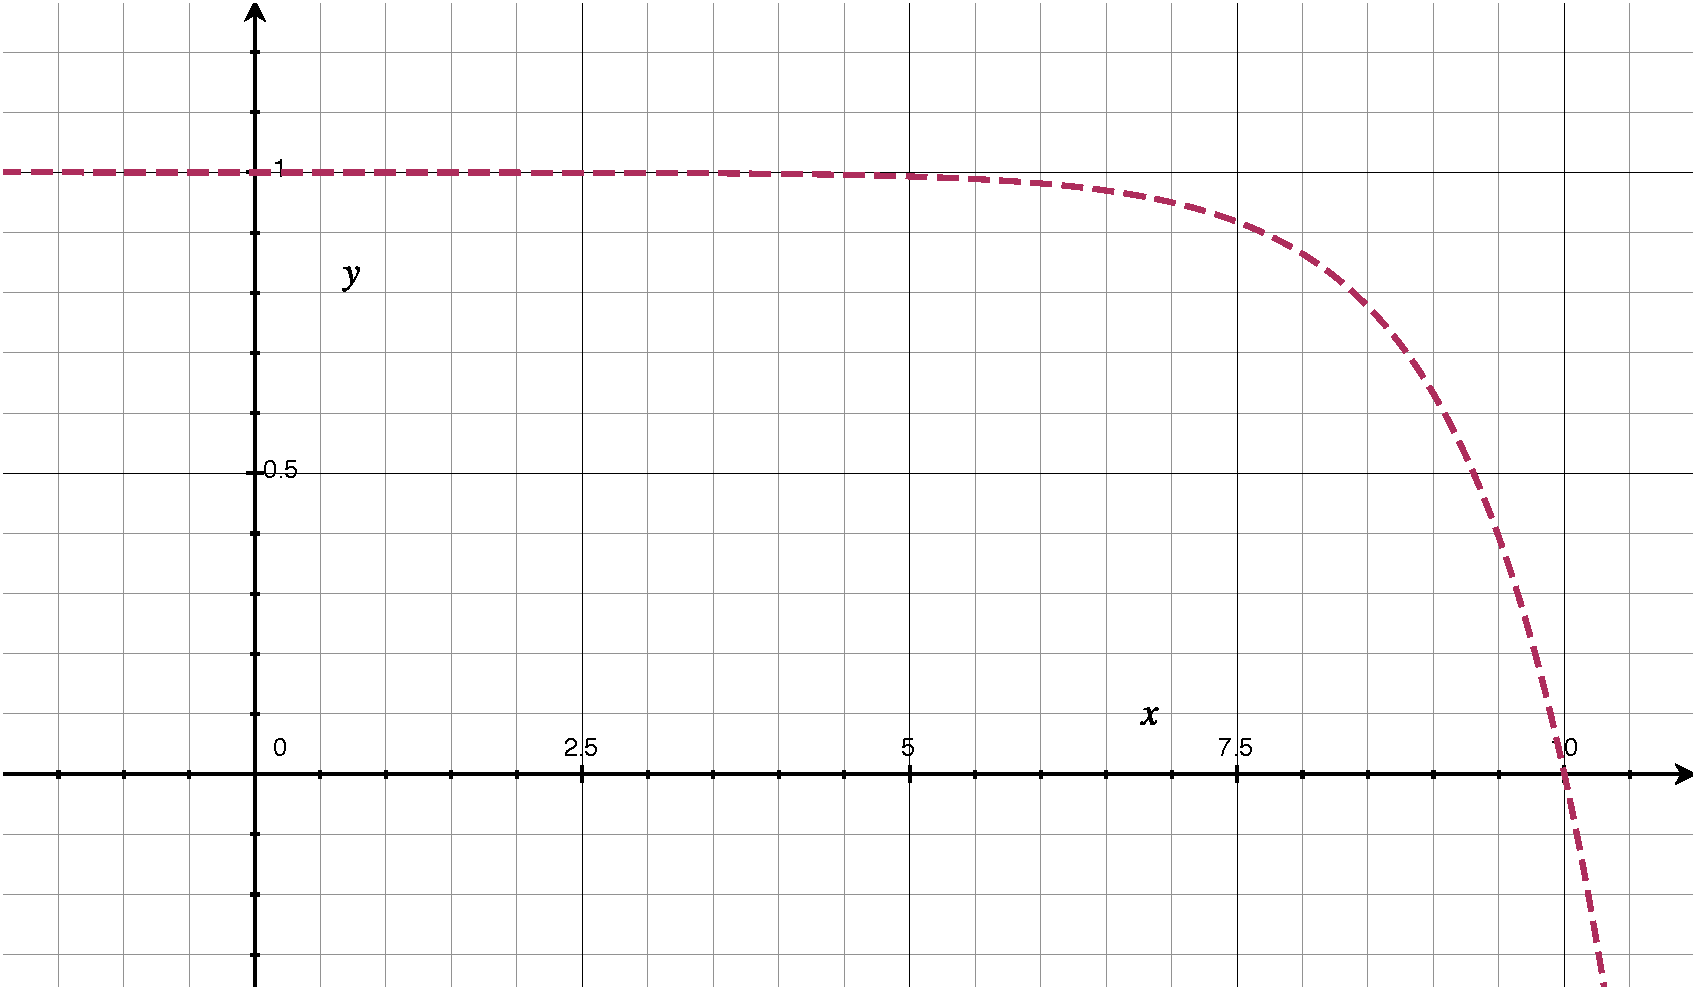
\includegraphics[width=0.9\textwidth]{u-power.pdf}
  \caption{Power applied at time $t$, for a race 10 seconds long.}
  \label{fig:power}
\end{figure}


\end{document}


